\documentclass{article}
\usepackage[utf8]{inputenc}

\usepackage[T1]{fontenc}
\usepackage[french]{babel}
\usepackage{amsmath}
\usepackage{amsfonts}
\usepackage{amssymb}
\usepackage{amscd}
\usepackage{amsthm}
\usepackage{physics}
\usepackage[left=2cm,right=2cm,top=2cm,bottom=2cm]{geometry}
\usepackage{textcomp,gensymb} %pour le °C, et textcomp pour éviter les warning
\usepackage{graphicx} %pour les images
\usepackage{subcaption}
\usepackage[colorlinks=true,breaklinks=true,
	citecolor=blue,
	linkcolor=blue,
	urlcolor=blue]{hyperref} % pour insérer des liens
\usepackage{epstopdf} %converting to PDF
\usepackage[export]{adjustbox} %for large figures

\usepackage{array}
\usepackage{dsfont}% indicatrice : \mathds{1}
\usepackage[dvipsnames]{xcolor}
\setcounter{tocdepth}{4} %Count paragraph
\setcounter{secnumdepth}{4} %Count paragraph
\usepackage{float}

\usepackage{array,tabularx}
\newcolumntype{L}[1]{>{\raggedright\let\newline\\\arraybackslash\hspace{0pt}}m{#1}}
\newcolumntype{C}[1]{>{\centering\let\newline\\\arraybackslash\hspace{0pt}}m{#1}}
\newcolumntype{R}[1]{>{\raggedleft\let\newline\\\arraybackslash\hspace{0pt}}m{#1}}

\title{Etude du premier modèle de Hindmarsh-Rose}
\author{Vincent Matthys Maureen Muscat Mariène Wan}
\date{\today}

\begin{document}

\maketitle





\section*{On fixe c = 1}
On a alors :
$$x_{Tr+} = 1 + \sqrt{\frac{2}{3}} \quad \text{et}\quad x_{Tr-} = 1 - \sqrt{\frac{2}{3}}$$




\begin{tabular}{|C{3.5cm} | C{2.2cm} | c  |}
\hline
Valeur de $I_{ap}$ & Nombre de points stat & Caractérisation des points \\
\hline
$I_{ap} \in ]-2, -1[$ & 1 & noeud stable \\
\multicolumn{3}{|c|}{\textcolor{red}{\textbf{Bifurcation pli}}} \\
$I_{ap} = -1 $ & 2 & noeud stable et \textbf{col-noeud} \\\hline
$I_{ap} \in ]-1, -0.9971[$ & 3 & noeud stable et \textbf{col et noeud stable} \\\hline
$I_{ap} \in ]-0.9971, -0.9264[$ & 3 & noeud stable et col et \textbf{foyer stable} \\
\multicolumn{3}{|c|}{\textcolor{Orange}{\textbf{Bifurcation Hopf}}} \\
$I_{ap} \in ]-0.9264, -0.816[$ & 3 & noeud stable et col et \textbf{foyer instable et cycle limite} \\\hline
\multicolumn{3}{|c|}{\textcolor{NavyBlue}{\textbf{Bifurcation homocline}}} \\
$I_{ap} \in ]-0.816, -0.0856[$ & 3 & noeud stable et col et \textbf{foyer instable} \\\hline
$I_{ap} = 0.0856$ & \multicolumn{2}{c|}{\textcolor{NavyBlue}{\textbf{Bifurcation homocline}}} \\\hline
$I_{ap} \in ]-0.0856, 5/27[$ & 3 & noeud stable et col et foyer instable et \textbf{cycle limite} \\\hline
$I_{ap} = 5/27 $ & 2 & \textbf{col-noeud} et foyer instable et cycle limite\\
\multicolumn{3}{|c|}{\textcolor{red}{\textbf{Bifurcation pli}}} \\
$I_{ap} \in ]5/27, 10[$ & 1 &  foyer instable et cycle limite \\
\hline
\end{tabular}
\vspace*{0,3cm}

Le cycle limite disparait aux alentours de  $I_{ap}=11,5$ et créer un foyer stable, ce foyer devient ensuite un noeud stable $I_{ap}=55,26$.


\paragraph*{}

Contrairement à $c = 2$, on a l'apparition de bifurcations homoclines (pour $I_{ap} = -0.
816$ et $I_{ap} = -0.0856$), faisant disparaître puis réapparaître le cycle limite stable.


Pour $I_{ap} = -0.817$, on peut voir dans la figure ci-dessous, à gauche, que les variétés stables et instable du col se superposent, on a donc une bifurcation homocline. De plus, au niveau du foyer instable, on peut observer l'existence d'un petit cycle limite. Celui-ci va disparaître pour $I_{ap} \geq -0.816$.
\begin{figure}[H]
    \centering

    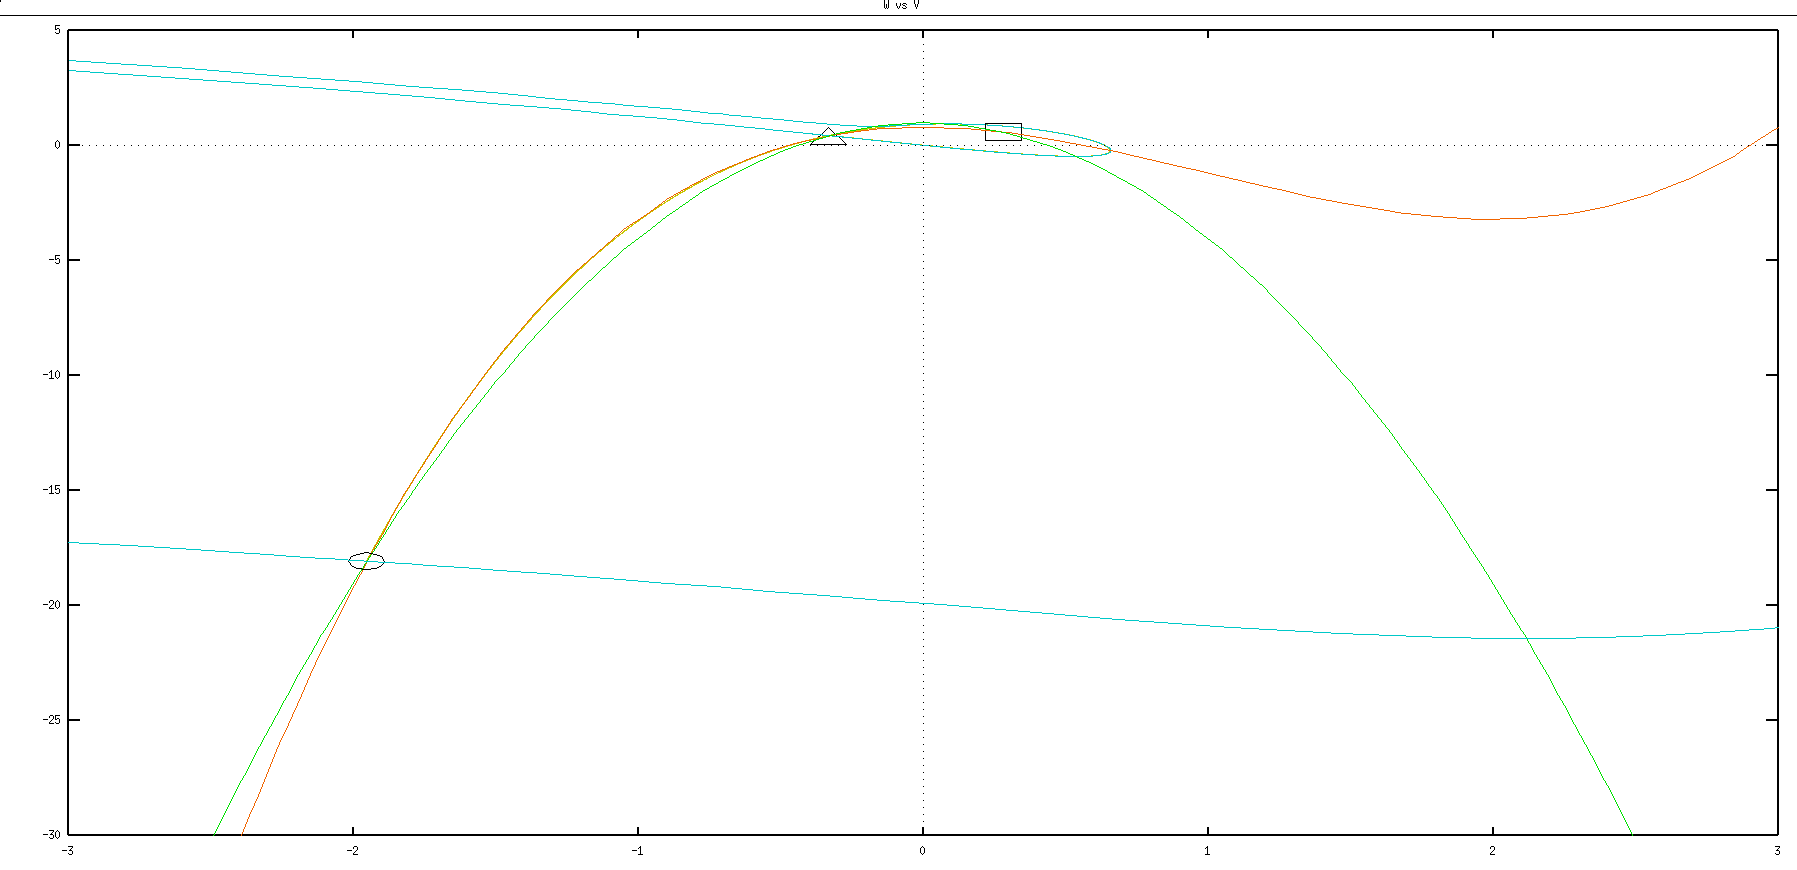
\includegraphics[width=0.45\textwidth]{I-0_817bis.png}
    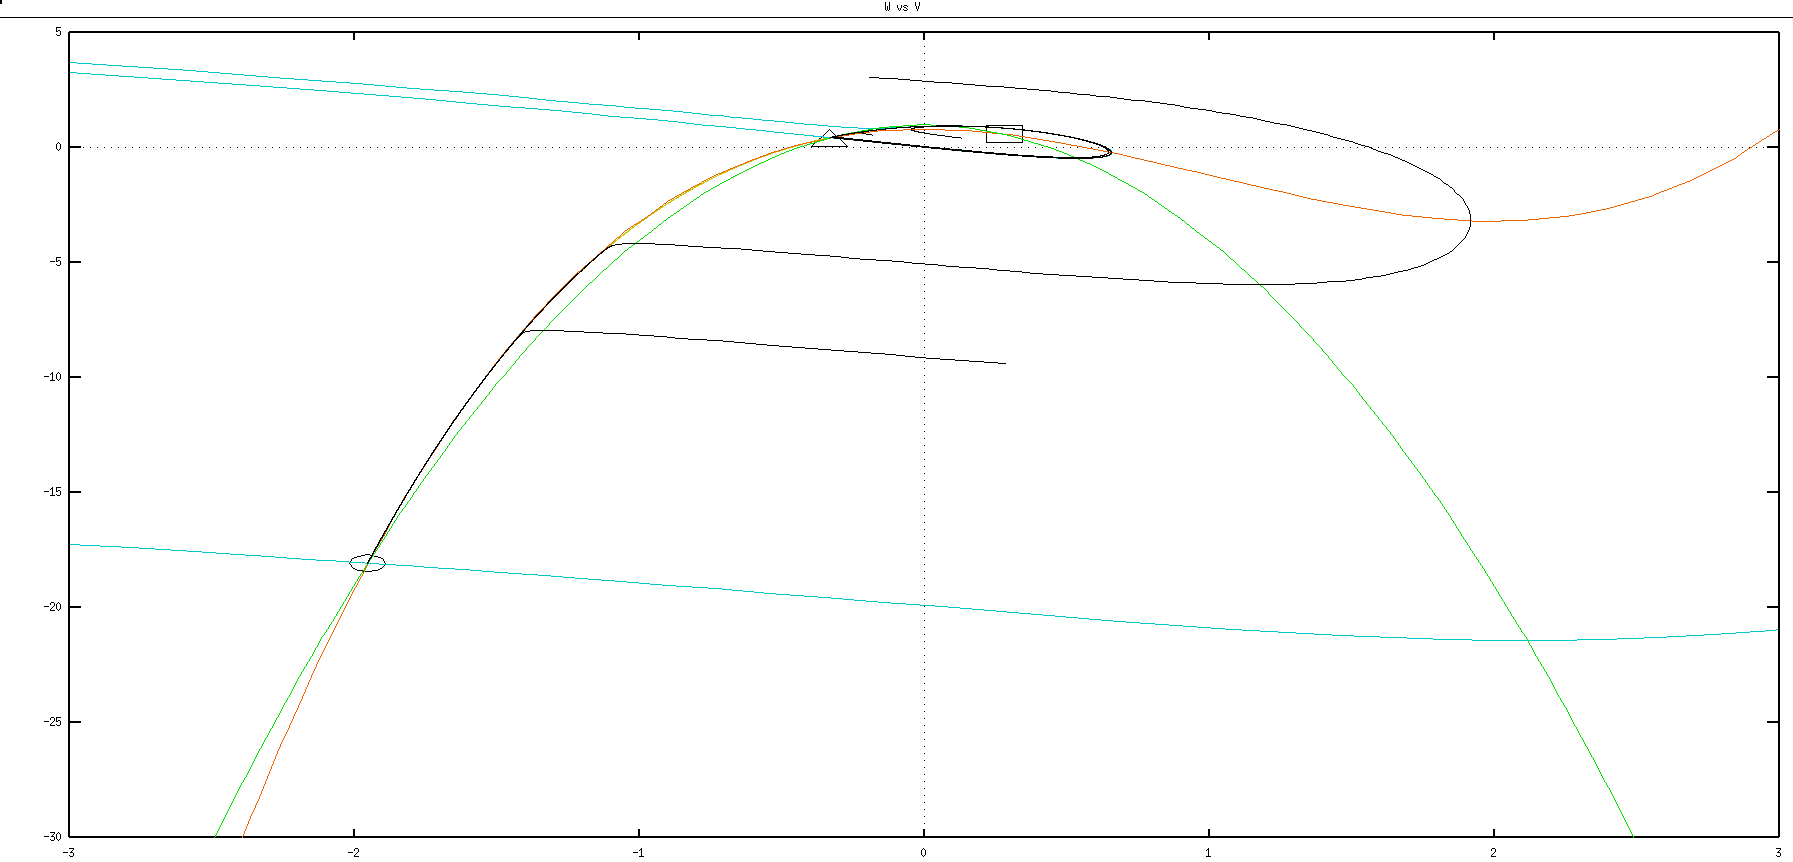
\includegraphics[width=0.45\textwidth]{I-0_817.png}

    \caption{Portrait de phase lorsque $I_{ap} = -0.817$ }
\end{figure}

Lorsqu'on a $I_{ap} = -0.5$, on n'a plus de cycle limite au niveau du foyer et de bifurcation homocline.
\begin{figure}[H]
    \centering
    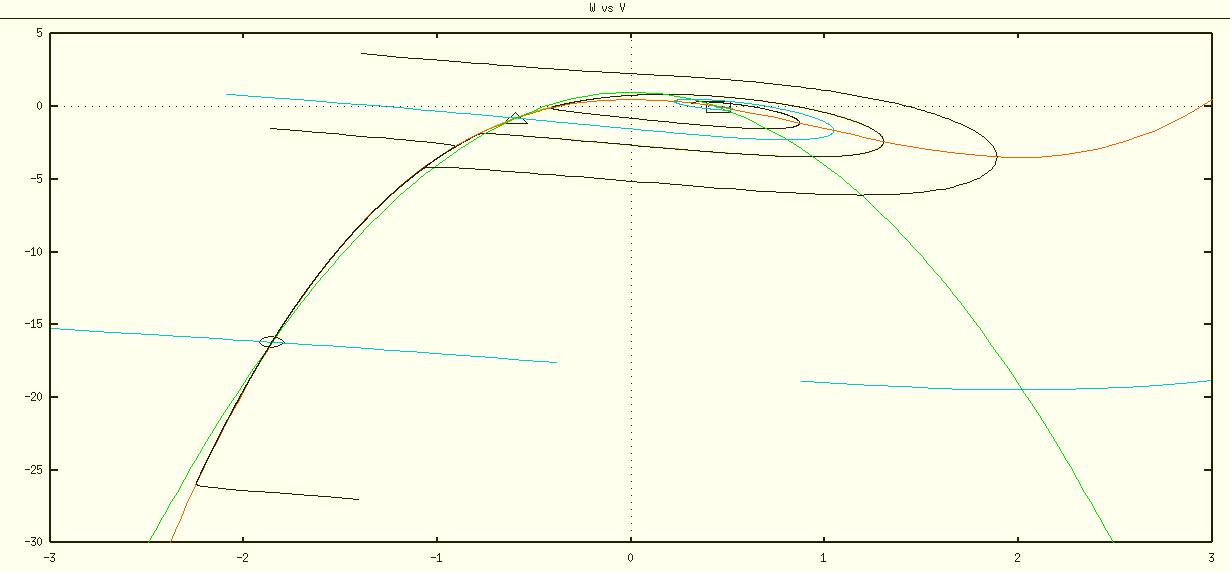
\includegraphics[width=0.8\textwidth]{I-0_5.png}
    \caption{Portrait de phase lorsque $I_{ap} = -0.5$ }
\end{figure}

Pour $I_{ap} = -0.008$, on a réapparition d'une bifurcation homocline, on peut observer sur la figure ci-dessous, que les variétés du col se superposent. Par ailleurs, on a aussi la réapparition d'un cycle limite, celui-ci va s'agrandir jusqu'à un certain point puis disparaitre  :
\begin{figure}[H]
    \centering
    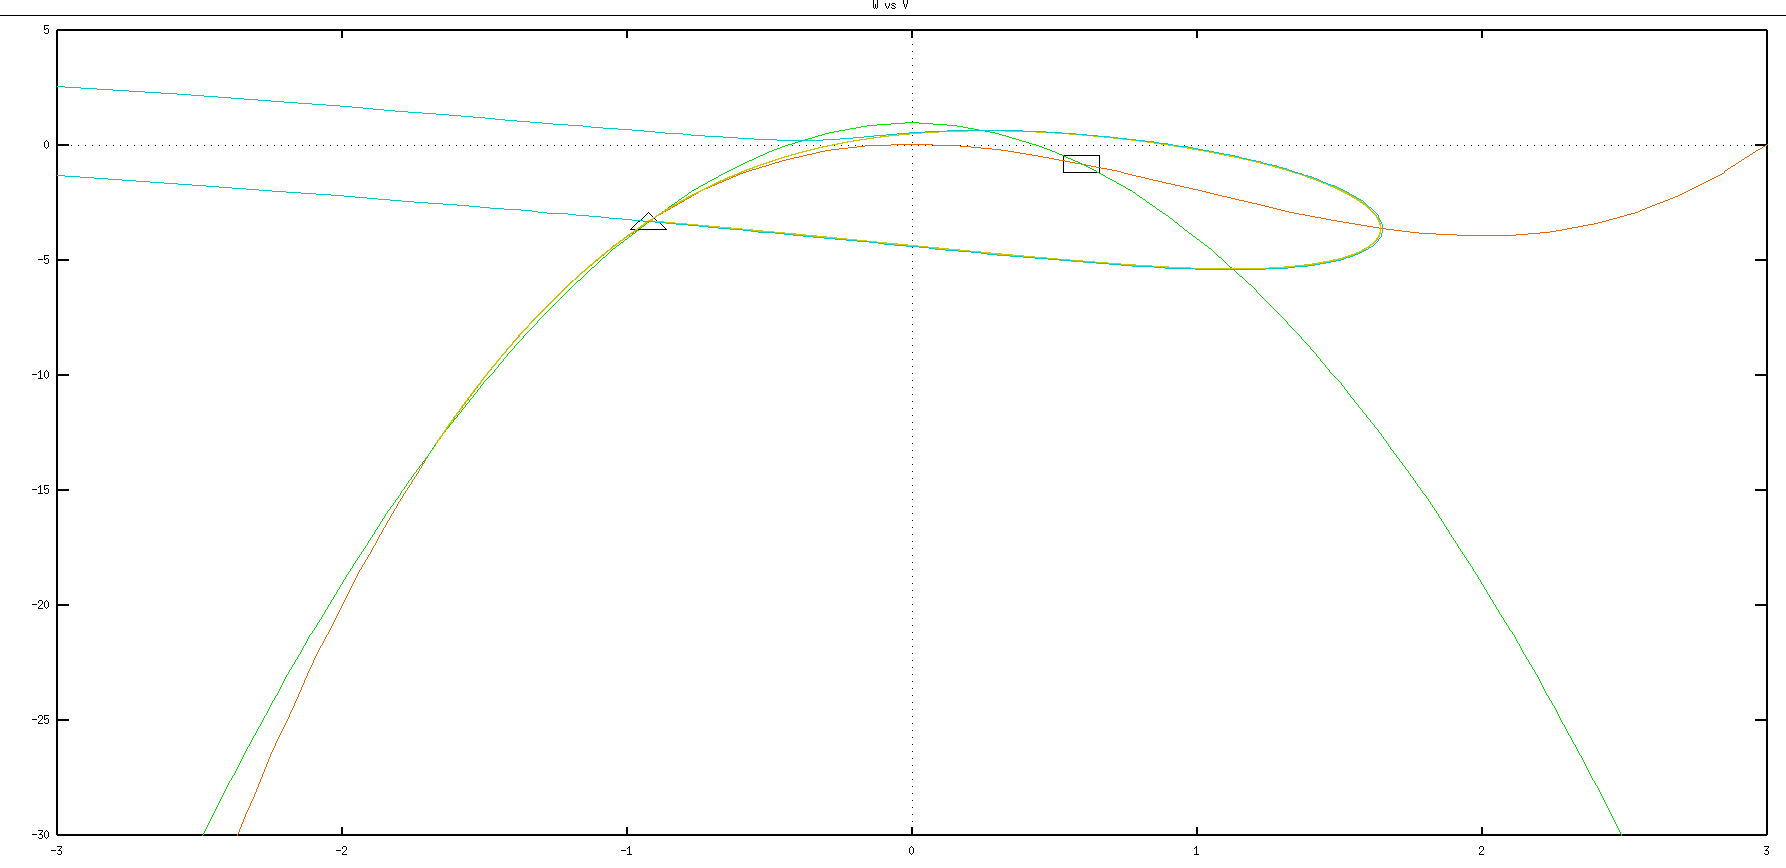
\includegraphics[width=0.5\textwidth]{I-0_008bis.png}
    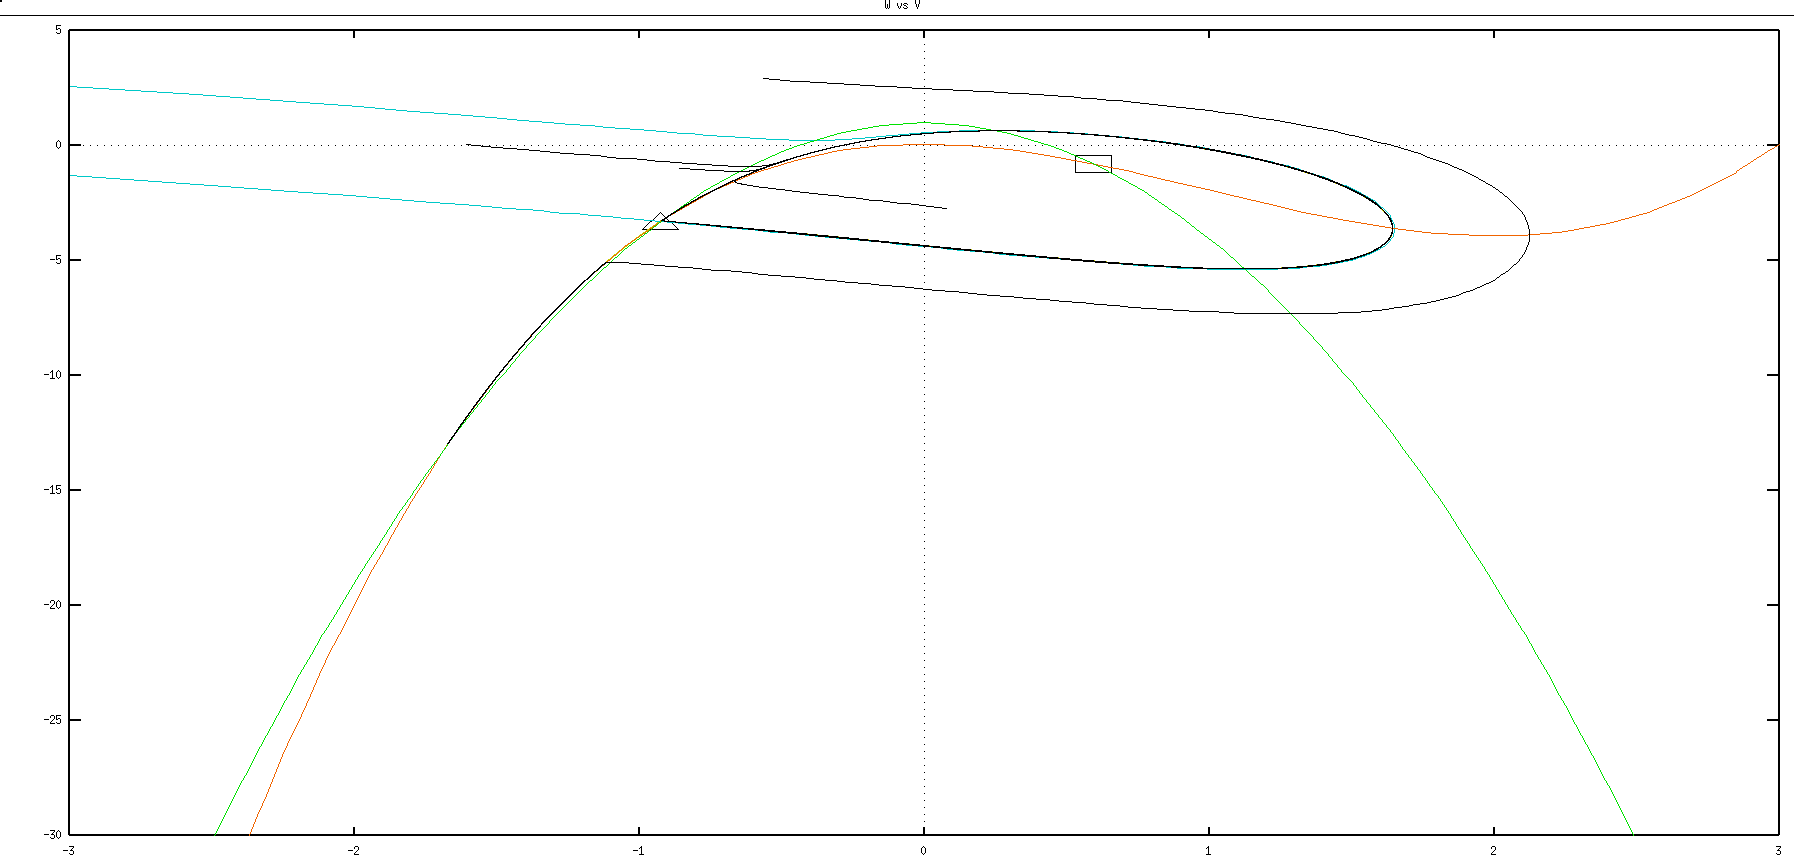
\includegraphics[width=0.5\textwidth]{I-0_008.png}
    \caption{Portrait de phase lorsque $I_{ap} = -0.008$ }
\end{figure}


Le système possède des régions de bistabilité :
\begin{itemize}
\item Pour $I_{ap} \in ]-1, -0,9264[$ avec 2 points stables,
\item Pour $I_{ap} \in ]-0,9264, -0,818[$ avec 1 point stable et un cycle limite
\item Pour  $I_{ap} \in ] -0,05, 5/27[$ avec 1 point stable et un cycle limite stable
\end{itemize}



\end{document}
